\chapter{\label{ch:5-result}Results}

\section{Digital literacy index - RQ1}

\begin{figure}
    \centering
    \caption{Screeplot of PCA - RQ1}
    \label{fig:screeplot_rq1}
    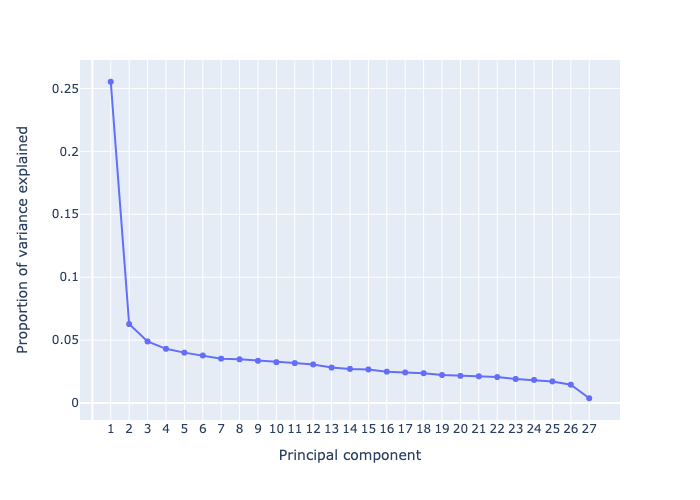
\includegraphics[width=\textwidth]{figures/pca_screeplot_q1.png}
\end{figure}


\begin{table}[h!]
    \centering
    \caption{Loadings of PC1 - RQ1}
    \label{tab:pc1_loadings_rq1}
    \begin{tabular}{llc}
        \toprule
        Feature & Description & Loading \\
        \midrule
        \textbf{Frequency of Internet usage} & 1 = every day, 6 = never & 0.280 \\
        & & \\
        \textbf{Hardware literacy} (devices) & 1 = yes, 0 = no & \\
        desktop &  & -0.094 \\
        laptop &  & -0.137 \\
        tablet &  & -0.121 \\
        smartphone &  & -0.245 \\
        other devices &  & -0.039 \\
        & & \\
        \textbf{Software literacy} (activities) & 1 = yes, 0 = no & \\
        emails &  & -0.258 \\
        video calls &  & -0.226 \\
        finding information &  & -0.218 \\
        finances &  & -0.247 \\
        shopping &  & -0.257 \\
        selling &  & -0.106 \\
        social networking &  & -0.178 \\
        news &  & -0.223 \\
        TV/radio &  & -0.219 \\
        music &  & -0.178 \\
        games &  & -0.082 \\
        e-books &  & -0.124 \\
        job application &  & -0.071 \\
        government services &  & -0.216 \\
        checking travel times &  & -0.248 \\
        satellite navigation &  & -0.229 \\
        buying public transport tickets &  & -0.167 \\
        booking a taxi &  & -0.088 \\
        finding local amenities &  & -0.231 \\
        controlling household appliances &  & -0.124 \\
        no online activities &  & 0.249 \\
        \bottomrule
    \end{tabular}
\end{table}


\begin{table}[h!]
    \centering
    \caption{Distribution of explanatory variable - RQ1}
    \label{tab:explanatory_variable_rq1}
    \begin{tabular}{lc}
        \toprule
        Digital literacy & Count \\
        \midrule
        Low & 994 \\
        High & 994 \\
        \bottomrule
    \end{tabular}
\end{table}

\section{Descriptive statistics - RQ1}


\begin{sidewaystable}[h!]
    \centering
    \footnotesize
    \caption{Descriptive statistics by digital literacy - RQ1}
    \label{tab:desc_stats_rq1}
    \begin{tabular}{llcc}
        \toprule
        Variables & Description & \multicolumn{2}{c}{Digital literacy} \\
        & & Low (N = 994) & High (N = 994) \\
        \midrule
        \textbf{Outcome variables} & & & \\
        Self-rated health & 1 = excellent, 5 = poor & 3.002 & 2.337 \\
        Physical health & 1 = yes, 0 = no & \\
        \hspace{0.5cm} High blood pressure &  & 0.468 & 0.308 \\
        \hspace{0.5cm} High cholesterol &  & 0.471 & 0.304 \\
        \hspace{0.5cm} Diabetes &  & 0.141 & 0.070 \\
        \hspace{0.5cm} Asthma &  & 0.114 & 0.100 \\
        \hspace{0.5cm} Arthritis &  & 0.477 & 0.318 \\
        \hspace{0.5cm} Cancer &  & 0.054 & 0.011 \\
        Mental health & & \\
        \hspace{0.5cm} Depression score & 0 = no symptom, 8 = all symptoms & 1.474 & 1.013 \\
        \hspace{0.5cm} Anxiety disorder & 1 = yes, 0 = no & 0.084 & 0.102 \\
        \hspace{0.5cm} Mood swings & 1 = yes, 0 = no & 0.020 & 0.014 \\
        & & & \\
        \textbf{Control variables} & & & \\
        Age &  & 74.408 & 64.655 \\
        Gender & 0 = male, 1 = female & 0.595 & 0.495 \\
        Marital status & proportion & & \\
        \hspace{0.5cm} Single &  & 0.064 & 0.079 \\
        \hspace{0.5cm} Married &  & 0.512 & 0.596 \\
        \hspace{0.5cm} Remarried &  & 0.100 & 0.151 \\
        \hspace{0.5cm} Separated &  & 0.008 & 0.009 \\
        \hspace{0.5cm} Divorced &  & 0.118 & 0.109 \\
        \hspace{0.5cm} Widowed &  & 0.198 & 0.056 \\
        Ethnicity & 0 = white, 1 = non-white & 0.023 & 0.048 \\
        Age left full-time education & 2 = never went to school, 8 = 19 or over & 5.101 & 6.704 \\
        Highest educational level & proportion & & \\
        \hspace{0.5cm} Degree or equivalent &  & 0.121 & 0.480 \\
        \hspace{0.5cm} HE below degree &  & 0.143 & 0.146 \\
        \hspace{0.5cm} A-level or equivalent &  & 0.098 & 0.142 \\
        \hspace{0.5cm} O-level or equivalent &  & 0.255 & 0.161 \\
        \hspace{0.5cm} CSE or equivalent &  & 0.050 & 0.005 \\
        \hspace{0.5cm} Foreign/other qualification &  & 0.097 & 0.044 \\
        \hspace{0.5cm} No qualification &  & 0.236 & 0.023 \\
        Employment status & 1 = in paid employment, 0 = not & 0.131 & 0.441 \\
        Household income (decile) & 0 = 1st decile, 9 = 10th decile & 3.263 & 5.753 \\
        Deprivation index & 0 = least deprived, 9 = most & 0.424 & 0.286 \\
        Memory & 1 = excellent, 5 = poor & 3.339 & 2.874 \\
        Numeracy index & 0 = lowest numeracy ability, 5 = highest & 3.423 & 4.217 \\
        Comprehension index & 0 = lowest comprehension ability, 4 = highest & 3.446 & 3.883 \\
        \bottomrule
    \end{tabular}
\end{sidewaystable}


\section{Main results - RQ1}

\begin{table}[h!]
    \centering
    \caption{IPTW estimate - Effect of digital literacy on health}
    \label{tab:iptw}
    \begin{threeparttable}
        \begin{tabular}{llc}
            \toprule
            Outcome & Description & IPTW \\
            \midrule
            Self-rated health & 1 = excellent, 5 = poor & \textbf{-0.326}*** \\
            & & [-7.353] \\
            & & \\
            Physical health & 1 = yes, 0 = no & \\
            High blood pressure &  & 0.002 \\
            &  & [0.065] \\
            High cholesterol &  & \textbf{-0.067}** \\
            &  & [-2.809] \\
            Diabetes &  & \textbf{-0.034}* \\
            &  & [-2.307] \\
            Asthma &  & \textbf{-0.042}** \\
            &  & [-2.787] \\
            Arthritis &  & -0.018 \\
            &  & [-0.758] \\
            Cancer &  & \textbf{-0.031}*** \\
            &  & [-4.068] \\
            & & \\
            Mental health & & \\
            Depression score & 0 = no symptom, 8 = all symptoms & \textbf{-0.292}*** \\
            & & [-3.887] \\
            Anxiety disorder & 1 = yes, 0 = no  & -0.018 \\
            &  & [-1.245] \\
            Mood swings & 1 = yes, 0 = no  & 0.009 \\
            &  & [1.757] \\
            \bottomrule
        \end{tabular}
        \begin{tablenotes}
            \footnotesize
            \item Notes: *** $p < 0.001$, ** $p < 0.01$, * $p < 0.05$. t-statistics are reported in square brackets.
        \end{tablenotes}
    \end{threeparttable}
\end{table}


\section{Robustness checks - RQ1}

\subsection{Strong ignorability}

\begin{figure}
    \centering
    \caption{Sensitivity analysis}
    \label{fig:sense}
    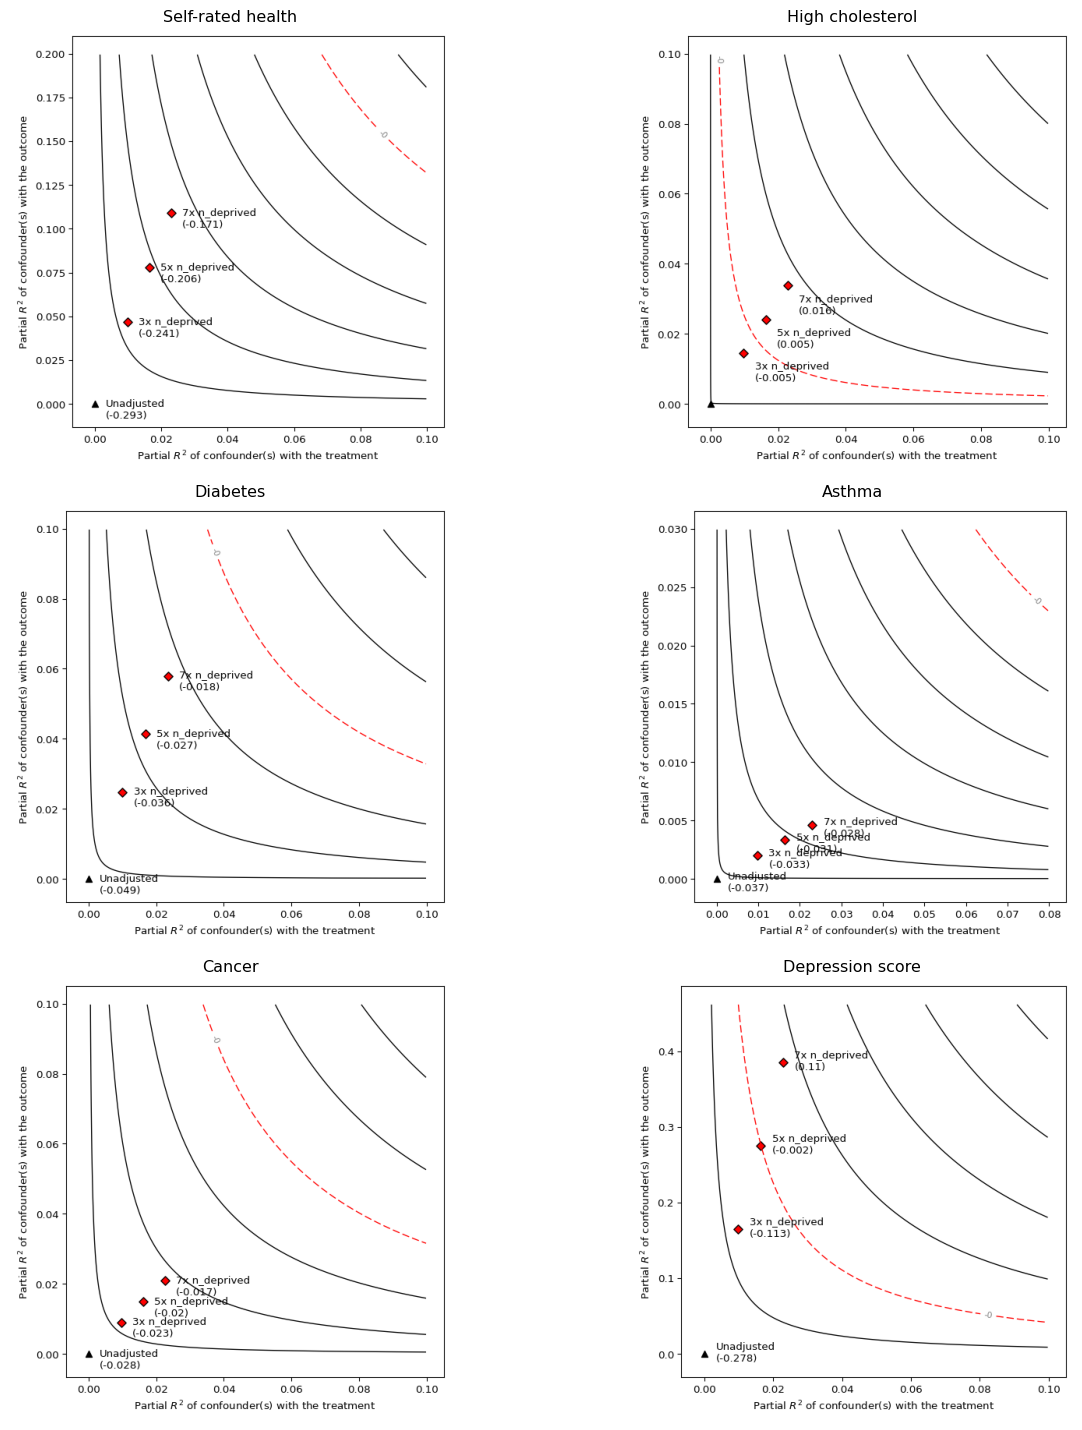
\includegraphics[width=\textwidth]{figures/sensitivity.png}
    \caption*{\footnotesize Notes: Points that reach the red dashed line indicate that the observed effect is nullified by the uncontrolled confounder.}
\end{figure}

\subsection{Positivity}



\section{Digital literacy index - RQ2}


\begin{figure}
    \centering
    \caption{Screeplot of PCA - RQ2}
    \label{fig:screeplot_rq2}
    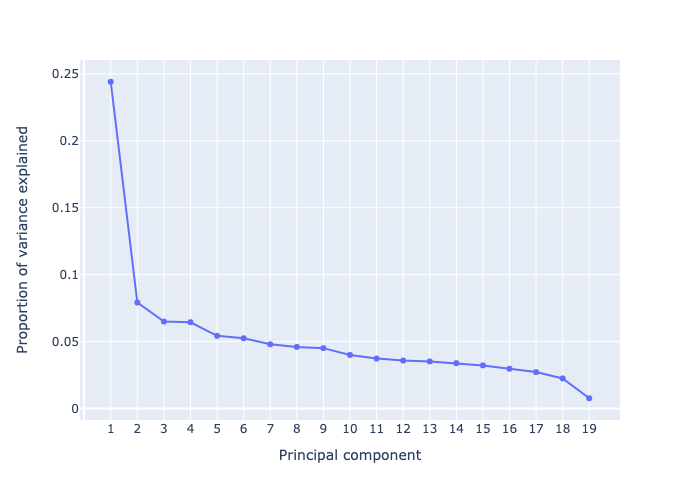
\includegraphics[width=\textwidth]{figures/pca_screeplot_q2.png}
\end{figure}

\begin{sidewaystable}[h!]
        \centering
        \caption{Loadings of PC1 - RQ2}
        \label{tab:pc1_loadings_rq2}
    
        \begin{subtable}[t]{0.4\textwidth}
            \centering
            \scriptsize
            \caption{Wave 9}
            \label{tab:pc1_loadings_w9_rq2}
            \begin{tabular}{llc}
                \toprule
                Feature & Description & Loading \\
                \midrule
                \textbf{Frequency of Internet usage} & 1 = every day, 6 = never & 0.357 \\
                & & \\
                \textbf{Hardware literacy} (devices) & 1 = yes, 0 = no & \\
                desktop &  & -0.124 \\
                laptop &  & -0.129 \\
                tablet &  & -0.143 \\
                smartphone &  & -0.243 \\
                other devices &  & -0.019 \\
                do not use any device &  & 0.320 \\
                & & \\
                \textbf{Software literacy} (activities) & 1 = yes, 0 = no & \\
                emails &  & -0.308 \\
                video calls &  & -0.176 \\
                finding information (learning) &  & -0.213 \\
                finding information (health) &  & -0.261 \\
                finances &  & -0.250 \\
                shopping &  & -0.269 \\
                selling &  & -0.107 \\
                social networking &  & -0.176 \\
                creating content &  & -0.084 \\
                news &  & -0.215 \\
                music &  & -0.214 \\
                games &  & -0.082 \\
                job application &  & -0.067 \\
                government services &  & -0.162 \\
                other online activities &  & -0.021 \\
                no online activities &  & 0.324 \\
                \bottomrule
            \end{tabular}
        \end{subtable}
        \hfil
        \begin{subtable}[t]{0.4\textwidth}
            \centering
            \scriptsize
            \caption{Wave 10}
            \label{tab:pc1_loadings_w10_rq2}
            \begin{tabular}{llc}
                \toprule
                Feature & Description & Loading \\
                \midrule
                \textbf{Frequency of Internet usage} & 1 = every day, 6 = never & 0.278 \\
                & & \\
                \textbf{Hardware literacy} (devices) & 1 = yes, 0 = no & \\
                desktop &  & -0.091 \\
                laptop &  & -0.134 \\
                tablet &  & -0.114 \\
                smartphone &  & -0.245 \\
                other devices &  & -0.042 \\
                & & \\
                \textbf{Software literacy} (activities) & 1 = yes, 0 = no & \\
                emails &  & -0.255 \\
                video calls &  & -0.224 \\
                finding information &  & -0.217 \\
                finances &  & -0.247 \\
                shopping &  & -0.255 \\
                selling &  & -0.107 \\
                social networking &  & -0.177 \\
                news &  & -0.225 \\
                TV/radio &  & -0.221 \\
                music &  & -0.183 \\
                games &  & -0.079 \\
                e-books &  & -0.124 \\
                job application &  & -0.072 \\
                government services &  & -0.218 \\
                checking travel times &  & -0.251 \\
                satellite navigation &  & -0.234 \\
                buying public transport tickets &  & -0.173 \\
                booking a taxi &  & -0.087 \\
                finding local amenities &  & -0.231 \\
                controlling household appliances &  & -0.126 \\
                no online activities &  & 0.243 \\
                \bottomrule
            \end{tabular}
        \end{subtable}
\end{sidewaystable}


\begin{table}[h!]
    \centering
    \caption{Distribution of explanatory variable - RQ2}
    \label{tab:explanatory_variable_rq2}
    \begin{tabular}{lcc}
        \toprule
         & Wave 10 - Low & Wave 10 - High \\
        \midrule
        Wave 9 - Low & 658 & 3 \\
        Wave 9 - High & 10 & 565 \\
        \bottomrule
    \end{tabular}
\end{table}


\section{Descriptive statistics - RQ2}

\begin{figure}
    \centering
    \caption{Health trends by digital literacy}
    \label{fig:desc_stats_rq2}
    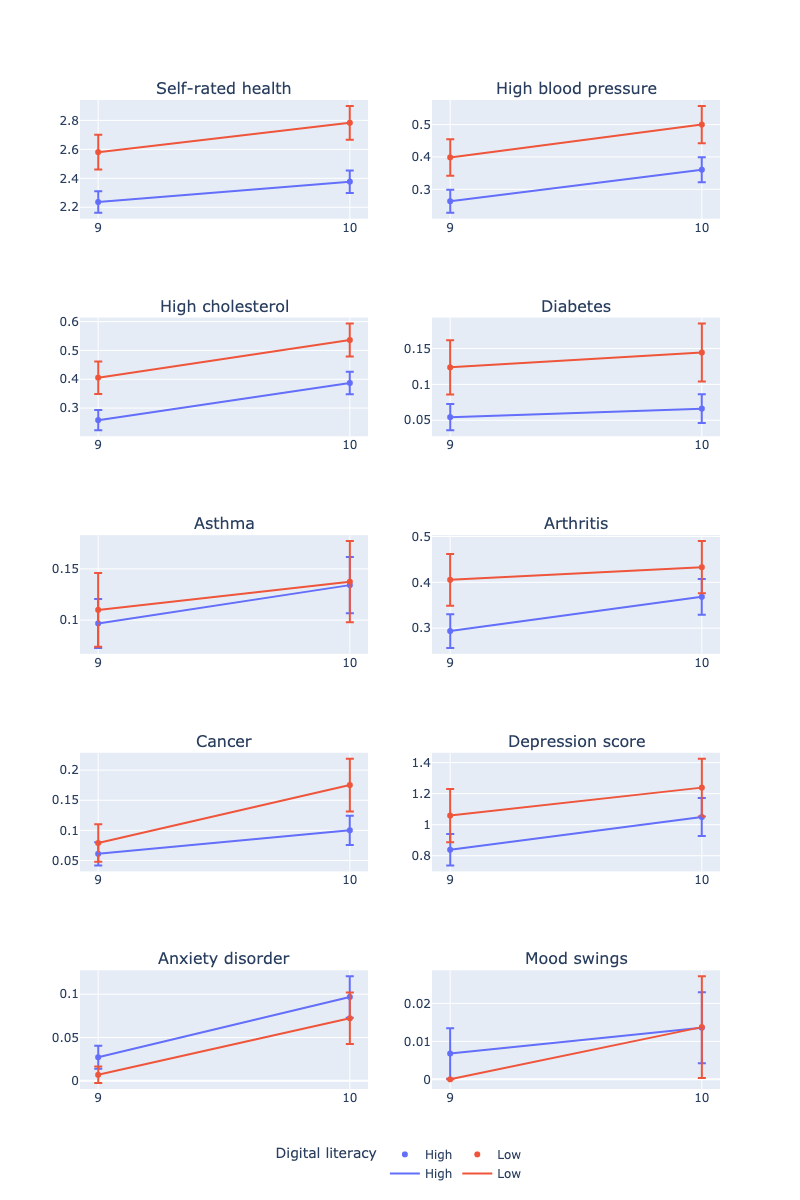
\includegraphics[width=\textwidth]{figures/desc_stats_q2.png}
    \caption*{Notes: The error bars represent 95\% confidence intervals.}
\end{figure}


\section{Main results - RQ2}


\begin{table}[h!]
    \centering
    \caption{DiD estimate - Impact of increased digitalisation on health disparities}
    \label{tab:did}
    \begin{threeparttable}
        \begin{tabular}{llc}
            \toprule
            Outcome & Description & Matching DiD \\
            \midrule
            Self-rated health & 1 = excellent, 5 = poor & \textbf{-0.207}*** \\
            &  & [-3.762] \\
            & & \\
            Physical health & 1 = yes, 0 = no & \\
            High blood pressure &  & -0.029 \\
            &  & [-1.523] \\
            High cholesterol &  & 0.002 \\
            &  & [0.061] \\
            Diabetes &  & \textbf{-0.044}*** \\
            &  & [-3.488] \\
            Asthma &  & 0.003 \\
            &  & [0.277] \\
            Arthritis &  & 0.01 \\
            &  & [0.562] \\
            Cancer &  & -0.026 \\
            &  & [-1.671] \\
            & & \\
            Mental health & & \\
            Depression score & 0 = no symptom, 8 = all symptoms & -0.115 \\
            &  & [-1.29] \\
            Anxiety disorder & 1 = yes, 0 = no & -0.011 \\
            &  & [-0.843] \\
            Mood swings & 1 = yes, 0 = no & \textbf{-0.013}** \\
            &  & [-2.845] \\
            \bottomrule
        \end{tabular}
        \begin{tablenotes}
            \footnotesize
            \item Notes: *** $p < 0.001$, ** $p < 0.01$, * $p < 0.05$. t-statistics are reported in square brackets.
        \end{tablenotes}
    \end{threeparttable}
\end{table}